\section{Návrh datového modelu}
\label{sub:data-model}

První krok\cite{data-model} při návrhu datového modelu je vypracování zadání a přesné vymezení datových entit, zatím určujeme pouze název a účel entity. Následně musíme definovat relace mezi daty, tedy popsat, jakým způsobem mezi sebou data interagují.

Druhým krokem je vytyčení atributů datových entit. U~atributu je třeba určit název, typ dat, která v~něm budou uložena, např. datum. Je také nutné určit zda bude atribut držet unikátní hodnoty, např. emailové adresy a zda je atribut povinný nebo zda může nést prázdnou hodnotu, tzv. \emph{null}\cite{null}.

Dalším krokem je adaptace tohoto obecného datového modelu, do modelu specifického pro prostředí, v~kterém budou data uložena, např. relační databáze. V~tomto kroku dojde k~materializaci relací mezi entitami na cizí klíče a intermediate tabulky\cite{intermediate-table}. Podle atributů vytvořených v~druhém kroku vytvoříme příslušné sloupce s~odpovídajícími datovými typy a omezeními. 

Posledním krokem, který nemusí nutně probíhat v~době návrhu, ale může být proveden dodatečně, je určení často využívaných dat a vytvoření tzv. \emph{indexů}\cite{index}. Ty slouží pro optimalizaci databázových dotazů a urychlení vyhledávání dat. \emph{Přílišné indexování může vést k~nárůstu velikosti databáze a zpomalení dotazů!}\cite{bad-indexing}

Datový model \bso{} je postaven kolem konceptu vystavovatele, z~implementačních důvodů reprezentováno tabulkou \emph{schools}.

\begin{figure}[H]
\centering
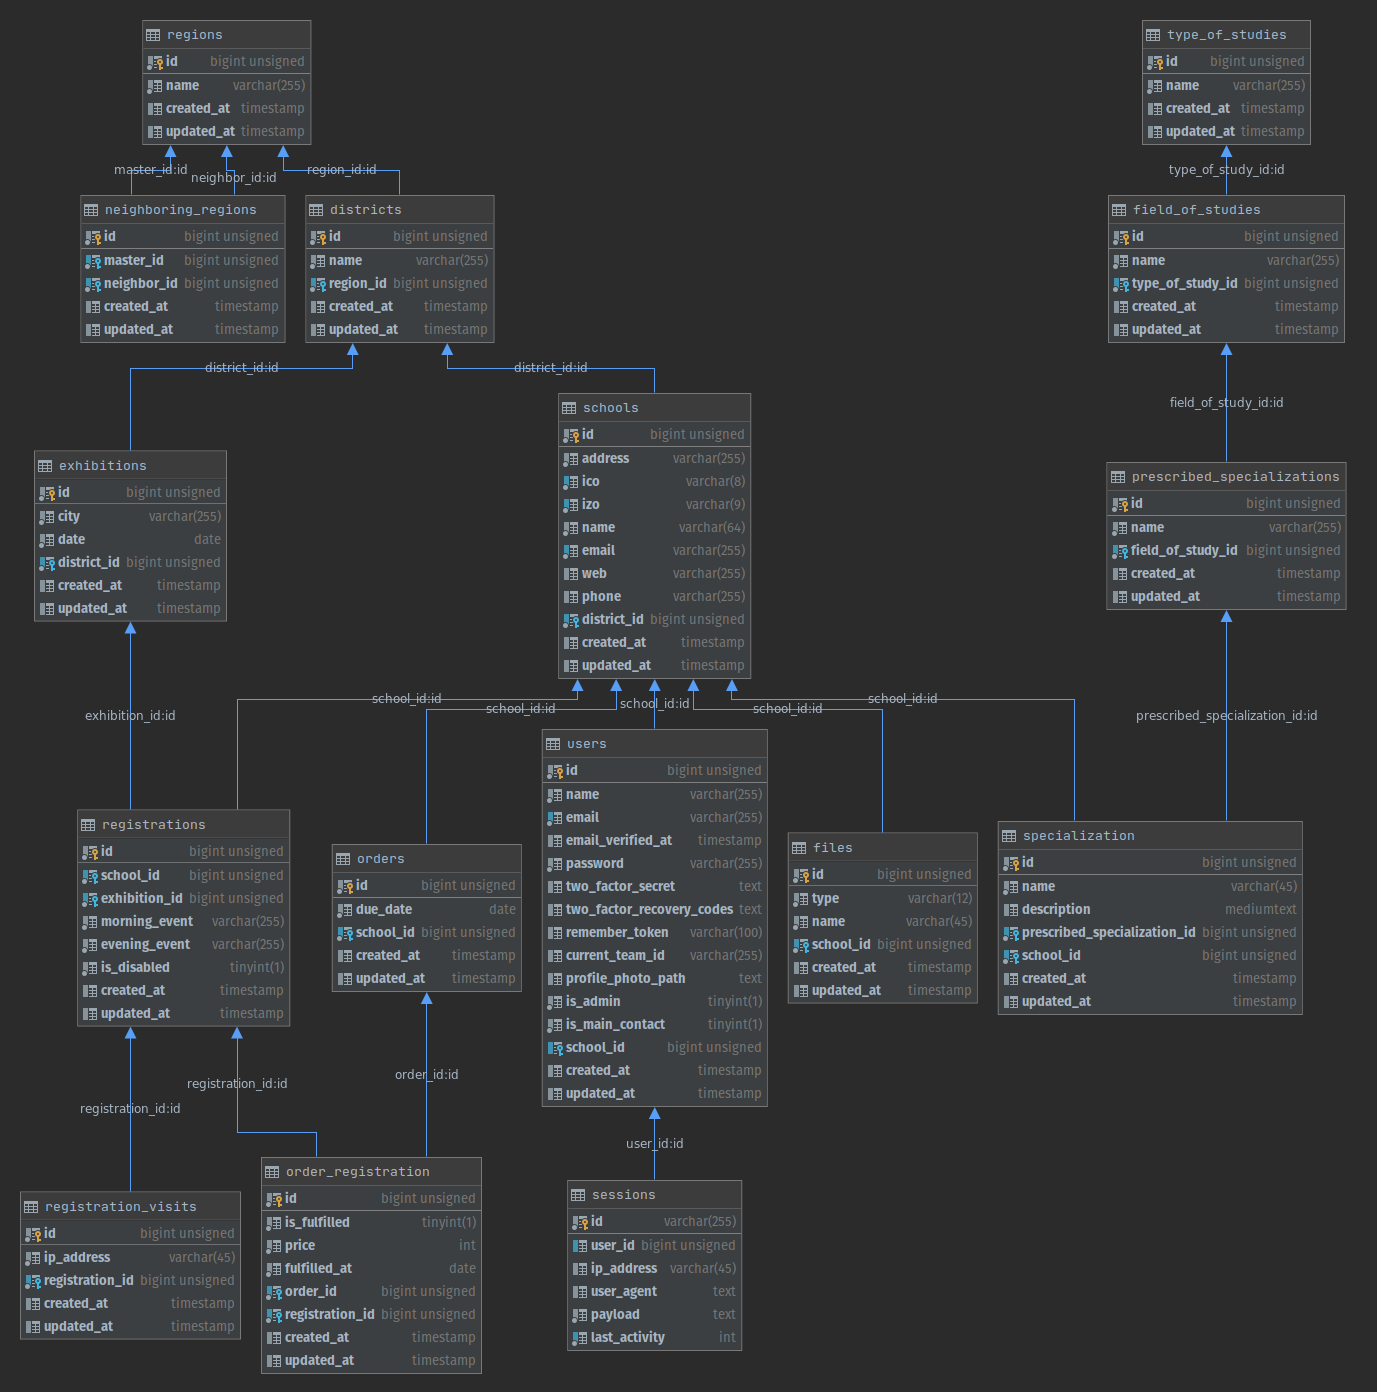
\includegraphics[width=\textwidth]{img/datovy-model-rijen-2020-2.png}
\caption{Datový model aplikace \bso{} k~říjnu roku 2020}
\label{fig:data-model-2020}
\end{figure}


Vystavovatelé jsou hlavní cílová skupina portálu. Mají možnost přihlásit se na výstavy a vložit krátký článek o~sobě,
případně o~svých oborech, s~podporou formátování za pomoci \acrshort{html} značek.
Portál umožňuje vystavovatelům nahrávat loga, informační brožury a obrázky, aby mohli zájemcům poskytnout maximální množství informací.
V~současné podobě projektu \bso{} existují tři typy vystavovatelů: školy, firmy a Úřady Práce České Republiky. 

Školy jsou hlavním typem vystavovatele. Mohou si vytvářet obory, které dále přiřazují k~oborům z~číselníku \acrshort{msmt}. To nám dovoluje poskytovat filtrování škol podle typu studia, zaměření a oborů samotných. Školy jsou také automaticky párovány s~výsledky maturitních zkoušek, výsledku soutěží zařazených do programu Excelence \acrshort{msmt} a k~inspekčním zprávám. Hlavní přínos portálu \bso{} pro školy je navázání kontaktu s~žáky 9. tříd a propagace. 

Druhým významným typem vystavovatele jsou firmy. Ty mohou vyjádřit svou podporu školám skrze funkcionalitu spolupráce. Kromě toho mají možnost seznámit zájemce se svou nabídkou pracovních pozic a stipendijních programů. Úřady práce mohou poskytovat nerozhodným žákům rady a dopomoci jim k~vybrání vysněného studijního oboru.
